% This is samplepaper.tex, a sample chapter demonstrating the
% LLNCS macro package for Springer Computer Science proceedings;
% Version 2.21 of 2022/01/12
%
\documentclass[runningheads]{llncs}
%
\usepackage[T1]{fontenc}
% T1 fonts will be used to generate the final print and online PDFs,
% so please use T1 fonts in your manuscript whenever possible.
% Other font encondings may result in incorrect characters.
%
\usepackage{graphicx}
% Used for displaying a sample figure. If possible, figure files should
% be included in EPS format.
%
% If you use the hyperref package, please uncomment the following two lines
% to display URLs in blue roman font according to Springer's eBook style:
%\usepackage{color}
%\renewcommand\UrlFont{\color{blue}\rmfamily}
%
\begin{document}
%
\title{A Review on Emotion Detection From Text: Opportunities and Challenges}
%
%\titlerunning{Abbreviated paper title}
% If the paper title is too long for the running head, you can set
% an abbreviated paper title here
%
\author{Anisur Rahman Mahmud\inst{1}\orcidID{19202103107} \and
Md Mubtasim Fuad\inst{1}\orcidID{19202103098} \and
Md Jahid Hasan\inst{1}\orcidID{19202103078} \and Md Minhazur Rafid \inst{1}\orcidID{19202103111
} \and Md Eusuf Khan \inst{1}\orcidID{19202103061} }
%
\authorrunning{Anisur et al.}
% First names are abbreviated in the running head.
% If there are more than two authors, 'et al.' is used.
%
\institute{Bangladesh University Of Business And Technology, Dhaka, Bangladesh }
%
\maketitle              % typeset the header of the contribution
%
\begin{abstract}
In this digital era, almost everyone can share their thoughts over the internet through texts in messages, posts or blogs and people often convey emotions of different sorts as well. Sometimes its about mental health, review about a bad product or simply opinions on different aspects of the modern world. Because of its massive popularity, emotion detection from text has become a burning topic for researchers. This review paper tries to provide understanding of different levels in various emotion models, different works that has been done in emotion identification from text and how it works along with introduction to various available datasets. Also how different models like LSTM, CNN, BERT and so on are utilized by researchers to provide better results in text based emotion detection is also discussed with their advantages and disadvantages. Finally this paper also points out different obstacles and challenges that lies in the study of emotion extraction from text. 

\keywords{Deep learning  \and Natural language processing \and Word embeddings \and LSTM \and Emotion Models.}
\end{abstract}
%
%
%
\section{Introduction}
Emotion detection from text is the process of extracting information from textual data using machine learning or deep learning methods. It can be viewed as an evolved specification of sentiment analysis. Sentiment analysis is not a new concept as there are hundreds of articles written about its methods and applications. Now emotion detection has numerous applications where it is used and continuously being improved to support more applications in the real world scenario. It started with NLP to enable computers to understand human speech~\cite{ref_url1}. Now the world moved to advanced step to understand emotions as well rather than only understand human speech to some extent.

Emotion identification is a means of extracting various human emotions. Emotions such as happy, sad, disgusted or angry. These emotions play a very important part in properly conveying the message. In today's world, people use social media applications extensively to communicate their feelings. Sometimes they express feelings, arguments or opinions on wide range of topics. Moreover people often provide feedback and reviews on different products for example book reviews. Now these reviews of books or any other products can be used to improve a product or service by vendors and service providers~\cite{ref4}. There is big amount of data present in the internet. So it has become important to transform these data into a more meaningful result so it can be used for decision making.

Emotion detection can also be applied in suicide notes or posts on social media to detect depression in subject~\cite{ref5}. Further more as internet availability increased, so did the amount of cyber bullying, hate speech in the internet. These hateful things can also be detected in social media or other platforms to provide healthy environment~\cite{ref3}. However it is also not as easy as it sounds. Language is prone to continuous evolution as there are new creations of slang words, sarcasm, use of emojis in sentences which makes it hard to predict the emotions accurately~\cite{ref6}. Still there are handful of models and methodologies to help solve these problems and be able to provide accurate results on various emotions. These models often include BERT, LSTM, NLP, Naive Bayes, linguistic regression etc. 

This review paper aims to serve as a guide to how different emotion detections work today with discussion of different approaches , concepts and dataset source availability for further researching this topic. It also points out end results of different methods undertaken by various researchers and their limitations and obstacles that were faced. The objectives of this paper are as follows
\begin{itemize}
\item Providing a review of the literature in the field of ED
\item Providing summery of the work that has been done
\item Discussing the shortcomings and opportunities
\end{itemize}

The rest of the article is presented as follows: sectin 2 introduces basic concept of emotion detection, emotion models. In section 3, current approaches used for properly extracting emotion are discussed along with different dataset sources available for research purposes. Section 4 outlines the results of various methods and unveil their limitations along with discussion how efficient different methods can be in different circumstances. Section 5 concludes the article.



%\begin{table}
%\caption{Table captions should be placed above the
%tables.}\label{tab1}
%\begin{tabular}{|l|l|l|}
%\hline
%Heading level &  Example & Font size and style\\
%\hline
%Title (centered) &  {\Large\bfseries Lecture Notes} & 14 point, bold\\
%1st-level heading &  {\large\bfseries 1 Introduction} & 12 point, bold\\
%2nd-level heading & {\bfseries 2.1 Printing Area} & 10 point, bold\\
%3rd-level heading & {\bfseries Run-in Heading in Bold.} Text follows & 10 point, bold\\
%4th-level heading & {\itshape Lowest Level Heading.} Text follows & 10 point, italic\\
%\hline
%\end{tabular}
%\end{table}


%\noindent Displayed equations are centered and set on a separate
%line.
%\begin{equation}
%x + y = z
%\end{equation}
%Please try to avoid rasterized images for line-art diagrams and
%schemas. Whenever possible, use vector graphics instead (see
%Fig.~\ref{fig1}).

%\begin{figure}
%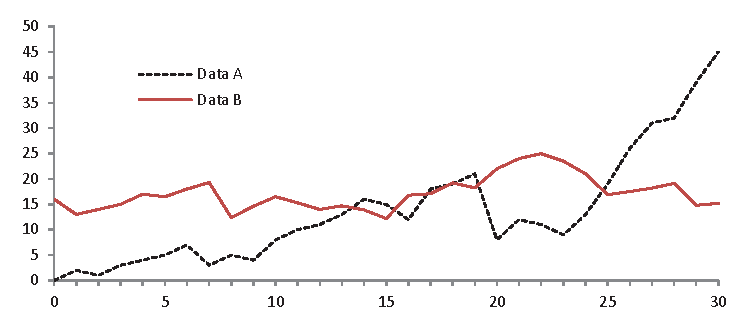
\includegraphics[width=\textwidth]{fig1.eps}
%\caption{A figure caption is always placed below the illustration.
%Please note that short captions are centered, while long ones are
%justified by the macro package automatically.} \label{fig1}
%\end{figure}

%
% the environments 'definition', 'lemma', 'proposition', 'corollary',
% 'remark', and 'example' are defined in the LLNCS documentclass as well.
%
%For citations of references, we prefer the use of square brackets
%and consecutive numbers. Citations using labels or the author/year
%convention are also acceptable. The following bibliography provides
%a sample reference list with entries for journal
%articles~\cite{ref_article1}, an LNCS chapter~\cite{ref_lncs1}, a
%book~\cite{ref_book1}, proceedings without editors~\cite{ref_proc1},
%and a homepage~\cite{ref_url1}. Multiple citations are grouped
%\cite{ref_article1,ref_lncs1,ref_book1},
%\cite{ref_article1,ref_book1,ref_proc1,ref_url1}.

\section{Background}
Basic understanding of emotion detection in general is necessary to grasp how it works and how various models in emotion detection play a very important role. So a discussion has been provided in its favour.
\subsection{Emotion Detection}
The base of human communication roots to emotions. These emotions play a very important role in human life. Emotion detection or identification refer to the method  of extracting emotional data such as feelings (sadness, happiness, anger etc) has been an interesting topic for researchers for a long time. A lot of different methods exist to automate the process of emotion identification. However, it is not an easy task as there are a lot of properties that must be taken into consideration in different situations. For example, facial expression plays a big role in conveying feelings of various kinds. Presence of occlusions, fluctuations in lighting, and changes in physical appearance all have an impact on showing emotions~\cite{ref7}. Physical changes for example heavy sweating, body temperature can also show signs of stress in human behaviour which can be taken into consideration when identifying emotions~\cite{ref8}. There's a big aspect in emotion which are expressed through movement of body parts as well for example, movement, body posture~\cite{ref9}. Taking all these into consideration, it is clear that emotions are conveyed through physical means a lot. Therefore it is not easy to automate the process of catching emotions from textual data. As more and more time passes, different slang words and sentences, sarcasm are also being part of the human language making the process more troublesome than before~\cite{ref6}. Furthermore there are more emotions to be taken under consideration as well. Emotions that includes feelings of happiness, sadness, disgust which could range from six to eight types of emotions depending on model used. 

\subsection{Emotion Models}
In order to implement the computing process to capture emotions, the definition of it first must be established properly. The basic concept of emotions was first introduced by Ekman~\cite{ref11} in the early 1970s. Although researchers try to classify emotions in different ways but there are no universally accepted emotion models. However,there are two types of generic emotion models which are often applied in computing processes which are discrete emotion model and dimensional emotion model.~\cite{ref11,ref12}.


\subsubsection{i. Discrete Emotion Model}

The discrete model defines emotions by placing them into limited categories or classes. One of the most widely used discrete emotion model is Ekman's six basic emotions. It is theorized that there are six emotions that originates from neural systems in human body because of how the person faces any certain circumstance. These emotions include anger, fear, disgust, happy, sad and surprise~\cite{ref11}. The development of Ekman's model is based on the hypothesis that human emotions are shared across races and cultures. However, different cultural backgrounds may show different interpretations of emotions~\cite{ref12}.

Another widely used discrete model is Plutchik's wheel model~\cite{ref10}. He classified emotions in eight ways such as joy, trust, fear, surprise, sadness, anticipation, anger and disgust. But they are related to each other and occur in opposite pairs and produces complex emotions. The eight emotions in opposite pairs are joy vs sadness, trust vs digust, anger vs fear, surprise vs anticipation. In Plutchik's wheel model, the stronger emotions occupy the center while the weaker emotions occupy the extremes as depicted in figure 1. These discrete emotions can be normalised into three kinds of polarity(positive, negative and neutral) which are often used in sentiment analysis.
\begin{figure}[ht!]
\centering
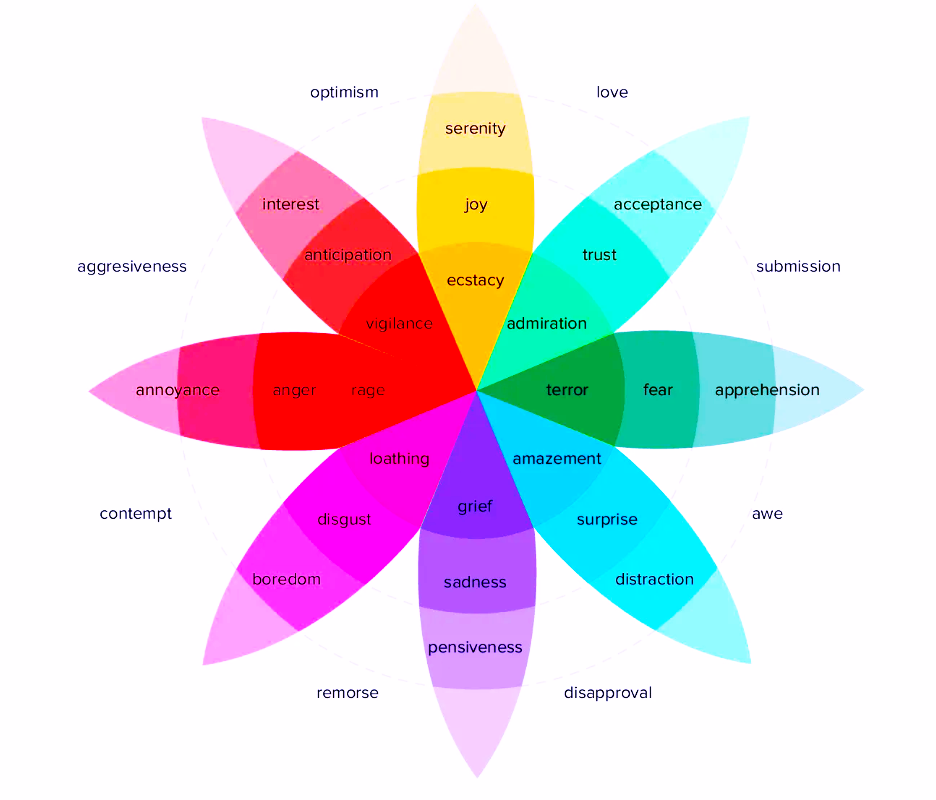
\includegraphics[scale=0.6]{plutchik}\label{Plutchik}
\caption{Plutchik's Wheel Model, indicating eight primary Emotions: anger, anticipation, joy, trust, fear, surprise, sadness and disgust where each emotion has a polar opposite emotion}
\end{figure} 



\subsubsection{ii. Dimensional Emotion Model}

Discrete emotion models comes with some challenges and to overcome those, many researchers have adopted the concept of multi-dimentional model. It proposes that emotions are not independent and there are relations between them hence the emotions are placed on dimensional space. One of the most recognized model of these approaches is Rusull's circumplex two dimentional model~\cite{ref14}. Here the model suggests that emotions can be shown with one dimension for arousal and one for valence. Arousal differentiates emotions by activations and deactivations and on the other hand, valence differentiates emotions by pleasantness and unpleasantness as depicted in figure 2.

\begin{figure}[ht!]
\centering
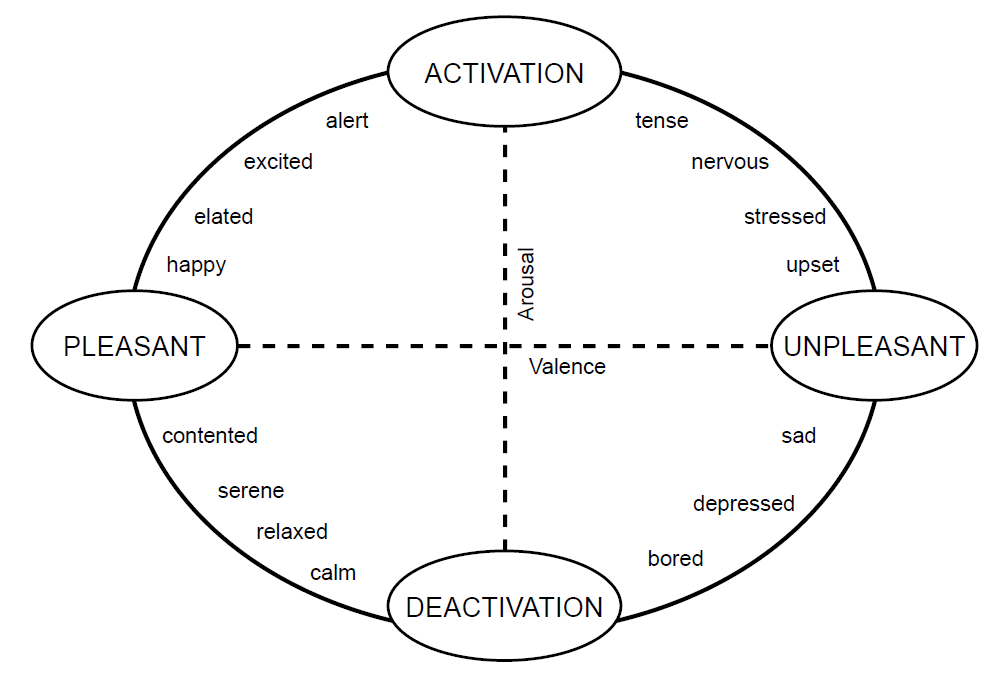
\includegraphics[scale=0.4]{russel}\label{Russel}
\caption{Valence-Arousal Model based on Russel's Circumplex Model, a dimensional emotion model where emotion is differentiated by arousal and valence. }
\end{figure} 

Another model was proposed by Russel and Mehrabian that present a 3 dimensional emotion model which is like circumplex model but there's an additional dimension named Dominance here. This dimension describes the degree to which the subject had control over their emotions~\cite{ref13,ref12}.

Of all the emotion models, the discrete models have been widely used for most emotion classification works due to its simplicity. But still it doesn't fully cover the extent of wide range of emotions from data as compared with the dimensional models. The dimensional models however are recommended in scenarios where similarities in emotions exist strongly.

\section{Resources And Approaches for Emotion Detection}
This section discusses different approaches to emotion detection taken by different researchers and their methods of execution. Also data collection is very important for perfectly detecting emotions. So different publicly available dataset is also presented here. 

\subsection{Datasets for Emotion Detection}
Datasets plays a very crucial role in developing the perfect emotion detection system. But there's a scarcity of publicly available resource for such research. There are a few structured datasets for emotion detection and a table containing their features, models and links is provided in Table 1.
One of the datasets here is EMOBANK~\cite{ref15,ref16} which has over 10000 sentences. The sentences were annotated in accordance to the Valence Arousal Dominance emotion representation model. A subset of the corpus have also been annotated according to Ekmans six basic emotions. The Workshop on Computational Approaches to Subjectivity, Sentiment, and SocialMedia Analysis (WASSA-2017)~\cite{ref19} data was constructed to detect emotion intensities in tweets. This dataset is also publicly available with four discrete emotions(joy,  anger, fear and sadness). Both training datasets and testing datasets are available. Multimodal EmotionLines Dataset (MELD)~\cite{ref17,ref18} has been created by enhancing and extending EmotionLines dataset. MELD contains the same dialogue instances available in EmotionLines, but it also encompasses audio and visual modality along with text. MELD has more than 1400 dialogues and 13000 utterances from Friends TV series. Emotions included here are anger, disgust, sadness, joy, surprise, fear and neutral. Emotion-Stimulas data~\cite{ref20} contains emotions as well as factors that cause those emotions. It has 820 sentences with both an emotion cause and an emotion tag. It also has a No Cause dataset which contains sentences marked with an emotion tag, which do not carry any emotion cause. This dataset contains 1594 instances marked with their emotion tag. Another dataset can be found from data.world where crowdflower released it under public license.In a variation on the popular task of sentiment analysis, this dataset contains labels for the emotional content (such as happiness, sadness, and anger) of texts. Hundreds to thousands of examples across 13 labels. DailyDialog~\cite{ref21} dataset was built by crawling dialogues from regular conversations. It contains a total of 13118 sentences annotated for neutral, , sadness, disgust, fear, happiness, surprise emotion labels.

\begin{table}
\caption{Available datasets for detecting emotion from texts}\label{tab1}
\resizebox{\textwidth}{!}{%
\begin{tabular}{|l|l|l|p{5cm}|}
\hline
Reference & Dataset & Model & Features\\
\hline
~\cite{ref_url2} & Emobank &  Dimensional & Obtained from cross cultural studies with 7665 sentences\\
\hline
~\cite{ref_url3} & Wassa 2017 &  Discrete & Constructed from tweets and annotated for joy, fear, sadness, and anger\\
\hline
~\cite{ref_url4} & MELD & Discrete & Obtained from quotes of a tv show called Friends\\
\hline
~\cite{ref_url5} & Emotion-Stimulas & Discrete & Dataset created from FrameNets containing 1594 emotion labelled sentence\\
\hline
~\cite{ref_url6} & Crowdflower & Discrete & Constructed from 39740 tweets in tweeter\\
\hline
~\cite{ref_url7} & DailyDialog & Discrete & Contains 13117 dialogues extracted from conversations\\
\hline
\end{tabular}
}
\end{table}

\subsection{Computational Approaches for Emotion Detection}
Emotion detection techniques can be divided into lexicon based approaches, machine learning approaches and deep learning based approaches. Lexicon based approaches rely on lexical resources such as lexicons, BOW(bag of words). Machine learning approaches apply ML algorithms based on linguistic related features. On the other hand, a more popular method nowadays is the deep learning approach. In deep learning approach, neural networks are used in attempt to stimulate AI to predict emotions with better accuracy.

In terms of machine learning approaches, Hossain et al~\cite{ref4} performed multinomial Naive Bayes on a dataset of 2000 bangla book reviews for emotion polarity detection. They added seven classifiers in their supervised machine learning model using Naive Bayes techniques to categorize the sentiment from reviews of books. They were successful in achieving accuracy upto 87\% and 84\% on validation and test datasets. However, the emotion extraction in their model did not take into consideration to classify more emotions rather than only positive and negative polarities. 

Fei H at el~\cite{ref22} proposed a model consisting of two components named a topic module and a capsule model. The topic module first learns latent topics keywords by reconstructing of the bag of words input via variational encoder. Then their capsule module captures features for each emotion from low level to high level. Later their developed algorithm captures relevant features for each emotion for capsule model to predict probability of each emotion label. Their usage of emotional model was dimensional. They reached microf1 score of 0.531.

For lack of performance of emotional analysis on short texts, Xu D at el~\cite{ref23} argued that even if other methods of emotion analysis may excel at full length documents, it lacks performance in microblog texts. They used deep learning method to propose their model. They used CNN that employs word2vec word embedding to train distributed word embedding fro every single word in mircroblog. Using a total of 80000 microblogs of dataset for algorithm training and testing. Their experiment shows that the word2vec word embedding provide 7\%, 6.9\% and 2.91\% higher accuracy than of SVM, RNN and LSTM respectively.

Chiorrini A et al~\cite{ref24} used twitter data for emotion recognition using BERT. Their proposal was to fine tune two BERT based classifications. They had to pre-process their datset as tweets often contains mentions, urls and retweets. Their model obtained accuracy upto 90\% in emotion detection and 92\% in sentiment analysis.

Sarcasm often proposes a challenge in emotion detection. In order to tackle the situation, Chauhan at el~\cite{ref6} developed a multi-task learning framework for detecting sarcsam and emotion of the speaker. They proposed two attention mechanics to better combine the information across the modalities to effectively classify sarcasm, emotion and sentiment. They first passed the input representation from all the three modalities through a fully connected layer to obtain the feature vector of length. These feature vectors are then forwarded to the aforementioned attention mechanisms. From there the representation is shared across five branches of the output layer. They claimed that the performance improvement in the framework over the state of the art is significant with 95\% confidence.

As the use of different embeddings greatly improves performance depending on dataset and circumstances used, Pepino at el~\cite{ref25} used BERT to recognize emotion from speech acoustic and text based features. For text based model, BERT was used for data extraction from text with additional fine tuning. Their experiments were preformed on the IEMOCAP and MSP PODCAST datasets. Here the fusion of audio and text based information leads to significant improvements of approximately 16\% on both datasets relative to using best sing modality.

Deep learning models are very handy in emotion detection related works. Wang at el~\cite{ref26} proposed an embedded recursive neural network for improving emotion detection. They aimed to do the potential and meaningful correlation among emotions from web news. They used two deep neural network models, CNN-LSTM2 (M1) abd CNN-LSTM2-STACK (M2) for this task. In both models, the length of an input text can be either short or long. They divided their calculation process into three parts where M1 is constructed into two parts and M2 is the third part where each part handles feature processing, emotion calculation and original feature attention respectively. Such methodology proved to provide accuracy upto 85\% in emotion detection. 

Yang at el~\cite{ref27} developed a model for detecting emotion expressed by an image-text post. Multi-channel Graph Neural Networks(MGNN) model was utilized here where it would contain three modules: the encoding module, the multi-GNN module and the multimodal interaction module. For text modality, they encoded words by GloVe to obtain the embedding vector and then obtain the text memory bank. For image modality, they extracted objects by YOLOv3 and extract scenes by VGG-Place. Finally obtaining the object and scene memory bank with pretrained ResNet. MGNN has excellent performance in sentiment analysis.

Use of different word embeddings improve performance of deep learning models. Polignano at el~\cite{ref28} compared the use of different word embedding in BiLSTM and CNN. They ran the models three times per dataset using one word embedding at a time. Among the word embeddings are Glove, FastText and Word2Vec. The results in their research showed promising accuracy in all emotional classes except for sadness reported in their paper.

LSTM is one of the popular deep learning models. Rashid at el~\cite{ref29} used LSTM to detect emotions in contextual conversations. They used word2vec and doc2vec embeddings.They used 15K tweet conversations and its responses. Their dataset was provided by SemEval 2019. Keras was used for pre-processing techniques. Their use of BiLSTM model took the embedding matrix as an input and the embedding matrix to be loaded in the embedding layer. They accomplished average of f1 score 69.63.

Krommyda at el~\cite{ref30} propose a fully pledged prototype for emotion detection from published social media posts. LSTM was used as a deep learning model. They downloaded tweets from tweeter and from there, a vocabulary was created using the most common words appearing. The vocabulary was used to transform each tweet into a vector. A total of 1.2 million annotated tweets was used as dataset. Accuracy of 91.9\% was achieved by the LSTM network.

Natural Language Processing Transformers is also used in emotion detection. Recently it was used in social robots by Graterol at el~\cite{ref31}. Their goal was to create a framework to allow social robots to detect emotions and store that information in semantic repository. The first version of their framework relies on a speech to text converter based on the google API and a python library, a neural network to label the emotions in texts based on NLP transformers and EMONTO, an ontology to represent emotions integrated with an ontology. They implement the whole pipeline taking into account only text and sound for a service robot in a museum getting feedback from users regarding the artworks. They were successful in making the robot system to able to recognize emotions from interactions with human.

Researchers often combine models together to achieve better result. Al-Omari at el~\cite{ref32} developed a system where they combined a fully connected neural network architecture and BiLSTM neural network to obtain performance results. They also extracted word contextual embedding from BERT base model. They collected feature vectors which feed different deep neural network architectures, feed-forward and LSTM model to obtain the desired predictions. Their model makes improvement by having F1 score of 0.789 over the baseline model provided by the Semeval 2019.

Chatterjee at el~\cite{ref33} used Bidirectional LSTM for their research in emotion detection. Their task proceeded in two phases. A training corpus of 30160 dialogues was provided at the beginning of phase 1. Their evaluation in this phase was done on an evaluation dataset of 2755 dialogues. Their final evaluation was carried out in phase 2 on a dataset of of 5509 dialogues. The highest rank they could achieve by the proposed system was 79.59 F1 micro score.

Machine learning approaches are also good in detecting emotions, specially in positive and negative intention from text. Sharma at el~\cite{ref34} used different machine learning algorithms like Naive Bayes, LR, LSTM and GRU to detect polar emotions. For RNN(LSTM and GRU), their model includes 3 different modules: data preparation, building their model and training the model. For LR and Nauve Bayes, datasets used contained thousands of tweets collected from twitter. Here sentiment for every tweet was labelled negative, positive and neutral. In their research, LSTM accuracy rate 74\%, GRU accuracy rate was 68\%, LR accuracy rate was 70\% and Naive Bayes accuracy rate was 60\%.

\section{Results, Discussion and Open Issues}

Here Table 2 provides a short summary of all the literature in the field of text based emotion detection as discussed in earlier. The work has been arranged according to the year of publication.

\begin{table}
\renewcommand{\arraystretch}{2}
\caption{Summary of advances by authors in emotion detection from text}\label{tab2}
\resizebox{\textwidth}{!}{%
\begin{tabular}{|l|l|l|l|}
\hline
Proposed Work & Approach & Dataset & F1 Score\\
\hline
Chatterjee at el~\cite{ref33} & LSTM &  SemEval 2019 & F1 0.795 \\
\hline
Polignano at el~\cite{ref28} & BiLSTM,CNN &  SemEval 2018 & F1 0.84 \\
\hline
Chauhan at el~\cite{ref6} & Hybrid Framework &  MUStARD & F1 0.725 \\
\hline
Xu D at el~\cite{ref23} & CNN &  Microblogs from Sina Weibo & F1 0.807 \\
\hline
Pepino at el~\cite{ref25} & BERT &  MSP-PODCAST & -- \\
\hline
Rashid at el~\cite{ref29} & LSTM & Tweets & F1 0.719 \\
\hline
Wang at el~\cite{ref26} & CNN-LSTM2 &  News Channel & -- \\
\hline
Fei H at el~\cite{ref22} & TE Capsule Network &  SamEval 2018 and RenCECps & Macro F1 0.576 \\
\hline
Al-Omari at el~\cite{ref32} & BiLSTM &  SamEval 2019 and RenCECps & F1 0.748 \\
\hline
Yang at el~\cite{ref27} & MGNN &  MVSA-Single-Multiple & 0.7270 \\
\hline
Krommyda at el~\cite{ref30} & LSTM &  Tweets & -- \\
\hline
Graterol at el~\cite{ref31} & NLP &  Conversation Data & Micro F1 0.636 \\
\hline
Chiorrini at el~\cite{ref24} & BERT &  amount of dataset & F1 0.91 \\
\hline
Hossain at el~\cite{ref4} & Naive Bayes &  data & Macro F1 0.81 \\
\hline
Sharma at el~\cite{ref34} & LR, LSTM, GRU &  Tweet & F1 0.68 \\
\hline
\end{tabular}
}
\end{table}

\begin{table}
\caption{Advantages and limitations of different approaches by researchers}\label{tab3}
\resizebox{\textwidth}{!}{%
\begin{tabular}{|l|p{5cm}|p{5cm}|}
\hline
Reference & Advantage & Limitation\\
\hline
Chatterjee at el~\cite{ref33} & \emph Was successful in identifying in four emotion \emph classes & One particular emotion \emph class had bad predictions than others\\
\hline
Polignano at el~\cite{ref28} & Suitable model for emotional intelligence capable systems  & Not good enough results for sad emotion class\\
\hline
Chauhan at el~\cite{ref6} & Proposed framework works on sentiment analysis, emotion and sarcasm detection as well & Use of smaller dataset\\
\hline
Xu D at el~\cite{ref23} & Showed that proposed model accuracy was 7\%,6.9\% and 2.91\% higher than SMV, RNN and LSTM respectively & More suitable for Chinese language\\
\hline
Pepino at el~\cite{ref25} & Showed that fusion of audio and text based information leads to significant improvement & Proposed model is very Complex\\
\hline
Rashid at el~\cite{ref29} & Hyper-parameters usage increased speed and quality of learning process & Use of stop words reduced accuracy\\
\hline
Wang at el~\cite{ref26} & Detection of correlation among emotions greatly reduced errors in emotion detection  & Trying shift of evolution law could have gotten better results\\
\hline
Fei H at el~\cite{ref22} & Proposed capsule model can capture rich features for corresponding emotions & Sometimes takes words out of context, giving wrong predictions\\
\hline
Al-Omari at el~\cite{ref32} & Use of BERT embedding in BiLSTM showed better performance & High model complexity\\
\hline
Yang at el~\cite{ref27} & Successfully detected text based emotion from images with 70\% accuracy & Data distribution in one dataset is unbalanced\\
\hline
Krommyda at el~\cite{ref30} & Emoji taken in consideration by algorithm improved performance & Low performance in some emotion classes\\
\hline
Graterol at el~\cite{ref31} & Framework can allow tour-guide robots that rely on speech to text converter to detect emotion & System is not robust\\
\hline
Chiorrini at el~\cite{ref24} & Model can be used for both sentiment \& emotion analysis while having 92\% \& 90\% accuracy in respective models  & Performance could be improved with bigger dataset\\
\hline
Hossain at el~\cite{ref4} & Proposed model outperforms LR, SVM \& SGD with 84\% accuracy on the test set  & Can only detect positive, negative \& neutral\\
\hline
Sharma at el~\cite{ref34} & Showed promising results in sentiment analysis & Models could have been better fine tuned\\
\hline
\end{tabular}
}
\end{table}

From the discussions carried out in this paper, it can be seen that accuracy, a lot of times, depend on various factors. For example, language representation and classification of emotions. Different languages also at times play a role in better extracting information or quite the opposite as seen in some papers where a model worked better on Chinese texts than English texts~\cite{ref23}. One of the reason for this kind of result could be the richness in dataset as well. Better pre-processed dataset can also improve a models efficiency in some cases. Also in case of classification of emotions, robust techniques for extracting emotions is also very necessary. Also rather than using a single model for emotion recognition, use of multiple models and later combining them to create fusion framework can be quite promising but also yields higher complexity. 

However, there are some issues that can be found in almost every research paper and should be discussed. Emotion detection can be most of the times successful but often there are false predictions in identifying some emotion classes. Most notably is sadness and disgust where often both emotions were misinterpreted. One was thought to be other by the models. This problem could be the use of slangs in sentences. Another reason could be the evolution of language. Sometimes words are used for an entirely different reason than its origin meaning. Thus the models would predict the wrong emotion if not the absolute opposite. Solving such issue can be quite troublesome and in some cases trying to solve such problems using stop words would often cause decreased accuracy~\cite{ref29} causing more negative impact on proposed model than good.

Emotion detection is very crucial as it has many applications in the real world. But one of the greatest obstacles in this case is the lesser amount of rich datasets availability, specially on other languages. The availability of rich resources in other language such as Bangla, Urdu or Hindi could greatly help researchers in further improving their models for applications to be used in regions where native languages are more heavily used rather than English. Also words and combination of words sometimes convey a lot of emotions than a completely structured sentence. Therefore publicly available datasets on more variety languages would greatly play an important part in advancing emotion detection technology and applications where emotion detection can be used.  

The models used and the approaches taken in emotion detection plays a big part in increasing effectiveness and performance. By studying different approaches, it can be seen that although different machine learning models can be used in terms of emotion recognition, deep learning models like BERT, BiLSTM, CNN completely outperforms others in accuracy and performance. Machine learning models are more suitable in detecting positivity or negativity of text. On the other hand, deep learning models allow extraction of more emotional features than ever possible using machine learning models. Now using deep learning models can improve performance but it can be greatly increased by fusing multiple models like BERT and LSTM together rather than using these models separately. It can also help in reducing wrong predictions in certain emotion classes. Yet the fusion techniques often appear to be very complex. These fusion of different models can be referred as hybrid models as well. Word embeddings also have a important role here. Using different word embeddings improve accuracy for certain models. Therefore it is highly recommended to check which word embedding technique runs well with proposed model giving better results.


\section{Conclusion}
In this paper, the current state of emotion detection from textual data was reviewed. The concept of text based emotion detection, different models and publicly available datasets were also introduced. The main approaches in emotion detection and how different researchers found innovative ways to tackle the task was also discussed here with the aim of better understanding this topic. The article further emphasised use of different datasets and limitations of some proposed models by other researchers. Finally ending the article on common issues discovered on a lot of the research documents which were focused on emotion detection from text.

%
% ---- Bibliography ----
%
% BibTeX users should specify bibliography style 'splncs04'.
% References will then be sorted and formatted in the correct style.
%
% \bibliographystyle{splncs04}
% \bibliography{mybibliography}
%
\begin{thebibliography}{8}
\bibitem{ref_url1}
Natural Language Processing, \url{https://en.wikipedia.org/wiki/Natural-language-processing}. Last accessed 1 September 2023

\bibitem{ref2}
Md. Yasin Kabir, Sanjay Madria, EMOCOV: Machine learning for emotion detection, analysis and visualization using COVID-19 tweets, Online Social Networks and Media, Volume 23, 2021, 100135, ISSN 2468-6964, https://doi.org/10.1016/j.osnem 2021.100135.

\bibitem{ref3}
Lippe P, Holla N, Chandra S, Rajamanickam S, Antoniou G, Shutova E, Yannakoudakis H. A multimodal framework for the detection of hateful memes. arXiv preprint arXiv:2012.12871. 2020 Dec 23.

\bibitem{ref4}
Hossain E, Sharif O, Moshiul Hoque M. Sentiment polarity detection on bengali book reviews using multinomial naive bayes. InProgress in Advanced Computing and Intelligent Engineering: Proceedings of ICACIE 2020 2021 Apr 16 (pp. 281-292). Singapore: Springer Singapore.

\bibitem{ref5}
Ghosh S, Ekbal A, Bhattacharyya P. A multitask framework to detect depression, sentiment and multi-label emotion from suicide notes. Cognitive Computation. 2022 Feb:1-20.

\bibitem{ref6}
Chauhan DS, Dhanush SR, Ekbal A, Bhattacharyya P. Sentiment and emotion help sarcasm? A multi-task learning framework for multi-modal sarcasm, sentiment and emotion analysis. InProceedings of the 58th Annual Meeting of the Association for Computational Linguistics 2020 Jul (pp. 4351-4360).

\bibitem{ref7}
Qazi AS, Farooq MS, Rustam F, Villar MG, Rodríguez CL, Ashraf I. Emotion Detection Using Facial Expression Involving Occlusions and Tilt. Applied Sciences [Internet]. MDPI AG; 2022;12:11797. Available from: http://dx.doi.org/10.3390/app122211797

\bibitem{ref8}
Zamkah A, Hui T, Andrews S, Dey N, Shi F, Sherratt RS. Identification of Suitable Biomarkers for Stress and Emotion Detection for Future Personal Affective Wearable Sensors. Biosensors [Internet]. MDPI AG; 2020;10:40. Available from: http://dx.doi.org/10.3390/bios10040040

\bibitem{ref9}
Wu C, Davaasuren D, Shafir T, Tsachor R, Wang JZ. Bodily expressed emotion understanding through integrating Laban movement analysis. arXiv preprint arXiv:2304.02187. 2023 Apr 5.

\bibitem{ref10}
Plutick R. Emotions and life: Perspective from psychology, biology, and evolution. 2002.

\bibitem{ref11}
Ekman P. Universals and cultural differences in facial expressions of emotion. InNebraska symposium on motivation 1971. University of Nebraska Press.

\bibitem{ref12}
Wang Y, Song W, Tao W, Liotta A, Yang D, Li X, Gao S, Sun Y, Ge W, Zhang W, Zhang W. A systematic review on affective computing: Emotion models, databases, and recent advances. Information Fusion. 2022 Jul 1;83:19-52.

\bibitem{ref13}
Bakker I, Van Der Voordt T, Vink P, De Boon J. Pleasure, arousal, dominance: Mehrabian and Russell revisited. Current Psychology. 2014 Sep;33:405-21.

\bibitem{ref14}
Russell JA. A circumplex model of affect. Journal of personality and social psychology. 1980 Dec;39(6):1161.

\bibitem{ref15}
Sven Buechel and Udo Hahn. 2017. EmoBank: Studying the Impact of Annotation Perspective and Representation Format on Dimensional Emotion Analysis. In EACL 2017 - Proceedings of the 15th Conference of the European Chapter of the Association for Computational Linguistics. Valencia, Spain, April 3-7, 2017. Volume 2, Short Papers, pages 578-585. Available: http://aclweb.org/anthology/E17-2092

\bibitem{ref16}
Sven Buechel and Udo Hahn. 2017. Readers vs. writers vs. texts: Coping with different perspectives of text understanding in emotion annotation. In LAW 2017 - Proceedings of the 11th Linguistic Annotation Workshop @ EACL 2017. Valencia, Spain, April 3, 2017, pages 1-12. Available: https://sigann.github.io/LAW-XI-2017/papers/LAW01.pdf

\bibitem{ref17}
S. Zahiri and J. D. Choi. Emotion Detection on TV Show Transcripts with Sequence-based Convolutional Neural Networks. In The AAAI Workshop on Affective Content Analysis, AFFCON'18, 2018.

\bibitem{ref18}
S. Poria, D. Hazarika, N. Majumder, G. Naik, E. Cambria, R. Mihalcea. MELD: A Multimodal Multi-Party Dataset for Emotion Recognition in Conversation. ACL 2019.

\bibitem{ref19}
Mohammad SM, Bravo-Marquez F. WASSA-2017 shared task on emotion intensity. arXiv preprint arXiv:1708.03700. 2017 Aug 11.

\bibitem{ref20}
Diman Ghazi, Diana Inkpen \& Stan Szpakowicz (2015). “Detecting Emotion Stimuli in Emotion-Bearing Sentences”. Proceedings of the 16th International Conference on Intelligent Text Processing and Computational Linguistics (CICLing 2015), Cairo, Egypt.

\bibitem{ref21}
Yanran Li, Hui Su, Xiaoyu Shen, Wenjie Li, Ziqiang Cao, and Shuzi Niu. 2017. DailyDialog: A Manually Labelled Multi-turn Dialogue Dataset. In Proceedings of the Eighth International Joint Conference on Natural Language Processing (Volume 1: Long Papers), pages 986–995, Taipei, Taiwan. Asian Federation of Natural Language Processing.

\bibitem{ref22}
Fei H, Ji D, Zhang Y, Ren Y. Topic-enhanced capsule network for multi-label emotion classification. IEEE/ACM Transactions on Audio, Speech, and Language Processing. 2020 Jun 10;28:1839-48.

\bibitem{ref23}
Xu D, Tian Z, Lai R, Kong X, Tan Z, Shi W. Deep learning based emotion analysis of microblog texts. Information Fusion. 2020 Dec 1;64:1-1.

\bibitem{ref24}
Chiorrini A, Diamantini C, Mircoli A, Potena D. Emotion and sentiment analysis of tweets using BERT. InEDBT/ICDT Workshops 2021 Mar 23 (Vol. 3).

\bibitem{ref25}
Pepino L, Riera P, Ferrer L, Gravano A. Fusion approaches for emotion recognition from speech using acoustic and text-based features. InICASSP 2020-2020 IEEE International Conference on Acoustics, Speech and Signal Processing (ICASSP) 2020 May 4 (pp. 6484-6488). IEEE.

\bibitem{ref26}
Wang X, Kou L, Sugumaran V, Luo X, Zhang H. Emotion correlation mining through deep learning models on natural language text. IEEE transactions on cybernetics. 2020 May 13;51(9):4400-13.

\bibitem{ref27}
Yang X, Feng S, Zhang Y, Wang D. Multimodal sentiment detection based on multi-channel graph neural networks. InProceedings of the 59th Annual Meeting of the Association for Computational Linguistics and the 11th International Joint Conference on Natural Language Processing (Volume 1: Long Papers) 2021 Aug (pp. 328-339).

\bibitem{ref28}
Polignano M, Basile P, de Gemmis M, Semeraro G. A comparison of word-embeddings in emotion detection from text using bilstm, cnn and self-attention. InAdjunct Publication of the 27th Conference on User Modeling, Adaptation and Personalization 2019 Jun 6 (pp. 63-68). 

\bibitem{ref29}
Rashid U, Iqbal MW, Skiandar MA, Raiz MQ, Naqvi MR, Shahzad SK. Emotion detection of contextual text using deep learning. In2020 4th International symposium on multidisciplinary studies and innovative technologies (ISMSIT) 2020 Oct 22 (pp. 1-5). IEEE.

\bibitem{ref30}
Krommyda M, Rigos A, Bouklas K, Amditis A. An experimental analysis of data annotation methodologies for emotion detection in short text posted on social media. InInformatics 2021 Mar 12 (Vol. 8, No. 1, p. 19). MDPI.

\bibitem{ref31}
Graterol W, Diaz-Amado J, Cardinale Y, Dongo I, Lopes-Silva E, Santos-Libarino C. Emotion detection for social robots based on NLP transformers and an emotion ontology. Sensors. 2021 Feb 13;21(4):1322.

\bibitem{ref32}
Al-Omari H, Abdullah MA, Shaikh S. Emodet2: Emotion detection in english textual dialogue using bert and bilstm models. In2020 11th International Conference on Information and Communication Systems (ICICS) 2020 Apr 7 (pp. 226-232). IEEE.

\bibitem{ref33}
Chatterjee A, Narahari KN, Joshi M, Agrawal P. SemEval-2019 task 3: EmoContext contextual emotion detection in text. InProceedings of the 13th international workshop on semantic evaluation 2019 Jun (pp. 39-48).

\bibitem{ref34}
Sharma T, Diwakar M, Singh P, Lamba S, Kumar P, Joshi K. Emotion Analysis for predicting the emotion labels using Machine Learning approaches. In2021 IEEE 8th Uttar Pradesh Section International Conference on Electrical, Electronics and Computer Engineering (UPCON) 2021 Nov 11 (pp. 1-6). IEEE.

%\bibitem{ref_lncs1}
%Author, F., Author, S.: Title of a proceedings paper. In: Editor,
%F., Editor, S. (eds.) CONFERENCE 2016, LNCS, vol. 9999, pp. 1--13.
%Springer, Heidelberg (2016). \doi{10.10007/1234567890}

%\bibitem{ref_book1}
%Author, F., Author, S., Author, T.: Book title. 2nd edn. Publisher,
%Location (1999)

%\bibitem{ref_proc1}
%Author, A.-B.: Contribution title. In: 9th International Proceedings
%on Proceedings, pp. 1--2. Publisher, Location (2010)


\bibitem{ref_url2}
EmoBank, \url{https://github.com/JULIELab/EmoBank}. Last accessed 28 August 2023

\bibitem{ref_url3}
WASSA-2017 Emotion Intensities(EmoInt), \url{http://
saifmohammad.com/WebPages/
EmotionIntensity-SharedTask.html}.
Last accessed 1 September 2023

\bibitem{ref_url4}
MELD Dataset, \url{https://github.com/declare-lab/MELD}. Last accessed 5 September 2023

\bibitem{ref_url5}
Emotion Stimulus, \url{https://www.site.uottawa.ca/\~diana/resources/emotion\_
stimulus\_data/}. Last accessed 30 August 2023

\bibitem{ref_url6}
CrowdFlower, \url{https://data.world/crowdflower/sentiment-analysis-in-text}.
Last accessed 1 September 2023

\bibitem{ref_url7}
DailyDialog, \url{https://aclanthology.org/I17-1099/}. Last accessed 1 September 2023


\end{thebibliography}
\end{document}
